\chapter{Methodology}
\label{chap:met}
\chaptermark{Methodology}

This chapter documents all engineering steps taken to build and exploit our
custom multimodal sEMG + hand-pose dataset. All code is MIT-licensed; the data
are provided free of charge with no usage restrictions.

\section{Why a New Dataset?}

\begin{itemize}
  \item \textbf{Hardware parity.} EMG2Pose uses 26 OptiTrack cameras and a
        proprietary CTRL-labs wristband -- out of reach for a \$1 000 budget.
  \item \textbf{Temporal realism.} Public corpora favour <10 s gesture clips;
        we require minutes-long, unscripted motion.
  \item \textbf{Storage efficiency.} Using a custom binary format, we
        reduce EMG2Pose`s session files to $\approx2.5\,\%$ of it's size, with no loss of
        information.
\end{itemize}

(An end-to-end tutorial that reproduces every step related to hardware soldering, dataset acquisition is included in the top-level README of \href{https://github.com/Senopiece/emg_hand_pose_dataset_capture/tree/v1.0}{this repository}\footnote{\url{https://github.com/Senopiece/emg_hand_pose_dataset_capture/tree/v1.0}}.)

\section{Four-Camera Hand-Pose Subsystem}

\subsection{Geometry and Calibration}

Four webcams (1280x800, 60 fps) are mounted around a
\SI{1.2}{\metre}$^{3}$ workspace -- three frontal views aimed at the palm and one
dorsal view. Accurate multi-view geometry is obtained with a \textit{radon
checkerboard}: an \emph{asymmetric} grid printed on \textbf{both} faces of an
A4 sheet, with extra anchor dots so the two patterns coincide perfectly when
held up to the light. Thanks to this dual-face design every camera can see a
valid checkerboard in the \emph{same} shot, eliminating the 180° ambiguity of
single-face boards.

\begin{enumerate}[label=\arabic*.]
  \item \textbf{Per-camera intrinsics}\\
        \verb|cv::findChessboardCorners| detects the pattern in live frames
        streaming from each webcam. Once every camera has logged
        $\ge12$ detections, \verb|cv::calibrateCamera| estimates the intrinsic
        matrix $K$ and distortion coefficients~$D$ individually
        (RMS reprojection error < \SI{0.3}{px}).

  \item \textbf{Pair-wise stereo calibration}\\
        One camera is designated the \emph{pivot}; by default the first index
        found in \texttt{cameras.def.json5}. For each remaining camera, the
        script runs \verb|cv::stereoCalibrate| against the pivot while
        \emph{fixing} the intrinsics from step 1.
        This yields a rotation $R$ and translation $T$ that map points from the
        pivot`s frame to the partner camera.

  \item \textbf{Write-out and visual check}\\
        All intrinsic blocks and $R\!T$ pairs are dumped to
        \texttt{cameras.calib.json5}. An optional preview window shows the
        rectified chessboard overlay on every camera so the operator can
        visually confirm alignment before recording.
\end{enumerate}

\noindent
The current implementation relies on direct \emph{pair-wise} overlaps with the
pivot camera; a note in the code highlights a future upgrade to bundle-adjust
\emph{all} pairs for even tighter global consistency. Nevertheless, the
stereo-against-pivot approach already provides sub-millimetre triangulation
accuracy at a working distance of \SI{50}{\centi\metre}, adequate for EMG-to-pose
learning.

\subsection{Landmark Triangulation \& Real-Time IK}

\begin{figure}[H]
    \centering
    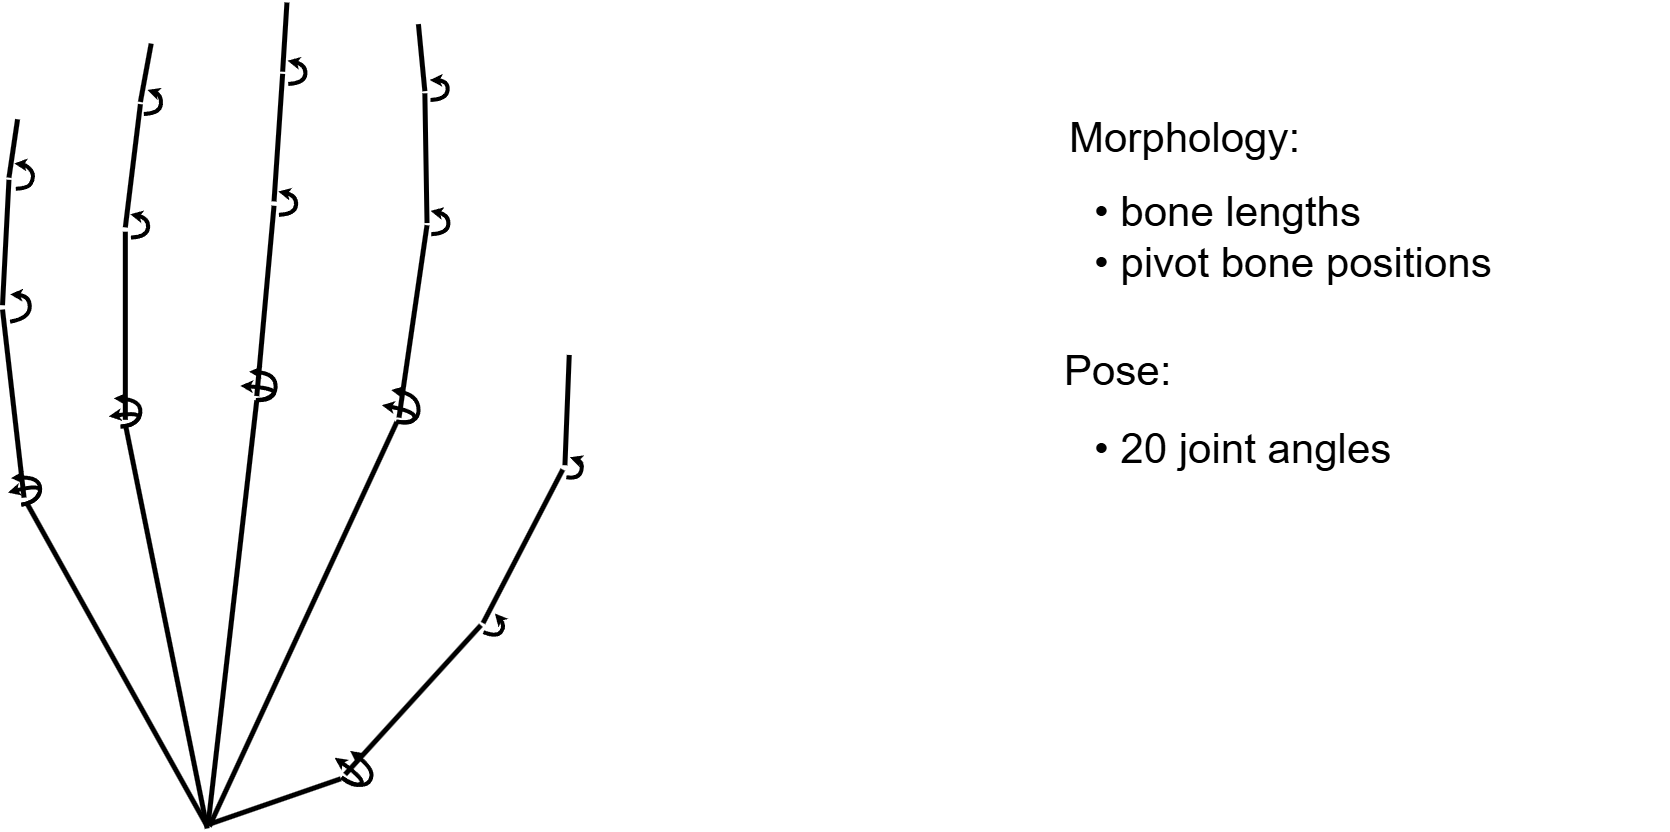
\includegraphics[width=1.0\textwidth]{kinematics.drawio.png}
    \caption{Kinematics.}
    \label{fig:kinematics}
\end{figure}

MediaPipe Hands detects 21 landmarks per retained frame (32 fps after
alignment). Multi-view triangulation yields 3-D key-points. A hand-crafted,
analytic inverse-kinematics solver enforces bone lengths and joint limits and works in real time.

Refer to \href{https://github.com/Senopiece/webcam_hand_triangulation/blob/v1.0/notebooks/kinematics.ipynb}{the notebook}\footnote{\url{https://github.com/Senopiece/webcam_hand_triangulation/blob/v1.0/notebooks/kinematics.ipynb}} to explore the kinematics more in-depth. 

\section{sEMG Acquisition Hardware}

TODO: image

\subsection{Electronics}
\begin{itemize}
  \item Four Bioelectronic-Circuit amps connected to Seeeduino Xiao (12-bit ADC).
  \item Sampling: \SI{2048}{Hz} x 4 channels.
  \item Streaming: USB 2.0 CDC, sustained $\approx \SI{2}{\mega\bit\per\second}$.
  \item No analogue or digital filtering at capture; any filtering is delegated
        to downstream models.
\end{itemize}

This setup is capable of capturing high-quality EMG signals and has shown it's usefulness in our previous work \cite{nasybullin2024methodology}.

\subsection{Electrode Montage}

\begin{figure}[H]
    \centering
    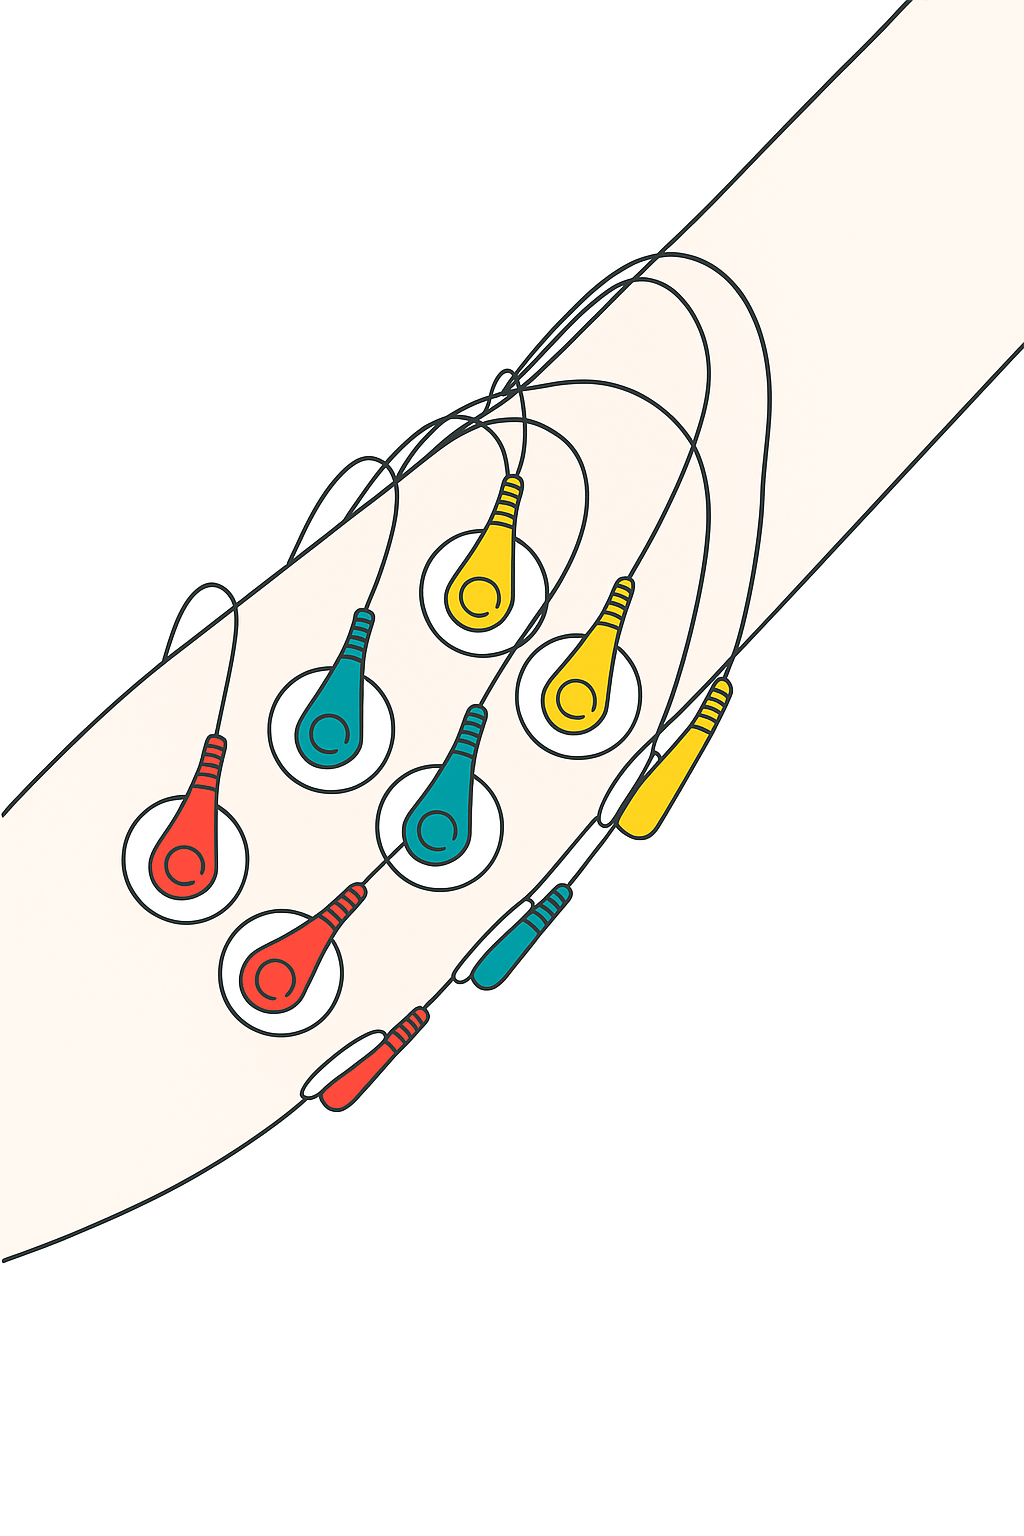
\includegraphics[width=0.4\textwidth]{electrodes.png}
    \caption{Electrode Placement.}
    \label{fig:electrodes}
\end{figure}

Twelve Ag/AgCl electrodes form four bipolar channels + reference to cover:

\begin{enumerate}[label=\alph*]
  \item \textbf{FDS} - \emph{Flexor Digitorum Superficialis}: the main finger-flexor mass on the palmar-ulnar side; activates when the fingers close.
  \item \textbf{FCR} - \emph{Flexor Carpi Radialis}: wrist flexor on the palmar-radial side; contributes to wrist flexion and radial deviation.
  \item \textbf{EDC} - \emph{Extensor Digitorum Communis}: dorsal-radial finger extensors; drives finger extension and assists in wrist extension.
  \item \textbf{ECU} - \emph{Extensor Carpi Ulnaris}: dorsal-ulnar wrist extensor; extends the wrist and produces ulnar deviation.
\end{enumerate}

\section{Dataset Infrastructure}
\begin{itemize}
    \item \textbf{Real-time I/O optimisations}.
          The capture software is build around a multithreaded
          worker-pool design. Careful use of mutexes and ring buffers resolved
          the synchronisation hazards that arise when high-rate EMG and video
          streams are written concurrently to disk.
    \item \textbf{Compact session format}.
          Each recording session is stored as a single ZIP archive containing
          \textbf{YAML metadata} plus proprietary binary segments for EMG and
          pose. Compared with an HDF5 dump of the same content, the archive
          shrinks disk usage by roughly \textbf{40x}. The public EMG2Pose
          corpus was re-encoded into this layout so that all datasets share one
          structure.
\end{itemize}

\subsection{Session Format}

\paragraph{Layout}

\begin{verbatim}
session.zip/
  metadata.yml
  recordings/
    1/segments/1 2 …
    2/segments/1 2 …
\end{verbatim}

\paragraph{Segment Binary Layout}

Each \texttt{segments/N} file contains a sequence of tuples:

\[
\bigl[
  [\underbrace{20\! \times\! \text{float32}}_{\text{pose}},
   \underbrace{64\!\times\!4}_{\text{EMG}}\text{ float32}],
  \dots,
  \underbrace{20\! \times\! \text{float32}}_{\text{sigma frame}}
\bigr]
\]

The final 20-value \emph{sigma frame} holds the last pose sample that is not coupled with EMG. That is representing the overall intuition of what each patch of the data time alignment is -- meaning that emg timestamp is always captured between pose frames.

\subsection{Synchronized Recording}

\begin{itemize}
  \item Cameras run at 60 fps; every second frame is kept 32 fps pose stream.
  \item Exactly 64 EMG samples (\SI{31.3}{ms}) align to each pose frame. The
        logger polls the \emph{latest} camera image at each 64-sample boundary.
  \item Timestamp jitter is negligible; no interpolation is
        applied for alignment.
\end{itemize}

\subsection{Quality Control}

TODO: image

The capture application shows

\begin{enumerate}[label=\alph*]
    \item \textbf{EMG oscilloscope}.
          Scrolling plots of each channel allow the operator to verify signal amplitude, baseline drift, and electrode contact before and during recording.
    \item \textbf{Session control panel}.
          A GUI window exposes start/stop buttons and a built-in timer that counts elapsed recording time, reducing annotation errors.
    \item \textbf{Interactive 3-D hand preview}.
          A interactive (rotate/zoom) viewer renders the triangulated skeleton so occlusions or tracking drop-outs can be spotted immediately.
\end{enumerate}

Immediate feedback helps catch loose electrodes or camera drop-outs.

\subsection{Re-encoding EMG2Pose}
Before training, the public EMG2Pose corpus is converted into this exact ZIP
layout using \href{https://github.com/Senopiece/hand_emg_regression/blob/v1.0/notebooks/convert_dataset.ipynb}{the Jupyter workflow}\footnote{\url{https://github.com/Senopiece/hand_emg_regression/blob/v1.0/notebooks/convert_dataset.ipynb}}. This notebook reads the original HDF5
files, extracts pose + EMG, and writes out ZIP packages with YAML metadata,
ensuring both corpora share an identical structure.

\subsection{Interpolation \& Resampling Strategy}

\paragraph{Pose formats.}
The loader supports two 20-angle representations:

\begin{itemize}
  \item \textbf{UmeTrack} -- the 20-DOF joint-angle vector used in the original
        EMG2Pose release. For strict comparability with that work, we keep the
        original \emph{linear} interpolation.
  \item \textbf{AnatomicAngles} -- our own 20-angle layout, reordered to match
        surface-EMG anatomy. Here we adopt \textbf{Akima splines}, which give
        smoother, overshoot-free trajectories well suited to biomechanical
        data.
\end{itemize}

\paragraph{Kernel benchmark.}
Five interpolation techniques were timed on a 250$\to$1000-frame up-sample test:

\begin{center}\small
\begin{tabular}{@{}lcc@{}}
\toprule
Scheme            & Time (ms) & Visual verdict \\ \midrule
Linear            & 1.0  & robotic, piecewise-constant velocity \\
\textbf{Akima}    & 6.4  & smooth, no overshoot (chosen) \\
Monotone cubic    & 8.3  & smooth but noticeably slower \\
Cubic spline      & 6.7  & severe overshoot at peaks \\
B-spline          & 9.3  & same overshoot issue, slowest \\ \bottomrule
\end{tabular}
\end{center}

Akima offers the best trade-off between speed and anatomical plausibility.

\paragraph{Loader-time resampling.}
Raw pose is stored exactly as captured at 32 fps.
When a model requests a different label rate (\{16, 32, 64, 128\} fps),
the dataset class resamples on the fly:

\begin{itemize}
  \item \textbf{UmeTrack} $\to$ linear interpolation,
  \item \textbf{AnatomicAngles} $\to$ Akima interpolation.
\end{itemize}

No interpolation is applied during live capture or camera-EMG alignment;
resampling is purely an offline, loader-side convenience.

\subsection{Inter-subject time-budget split.}

\begin{figure}[H]
    \centering
    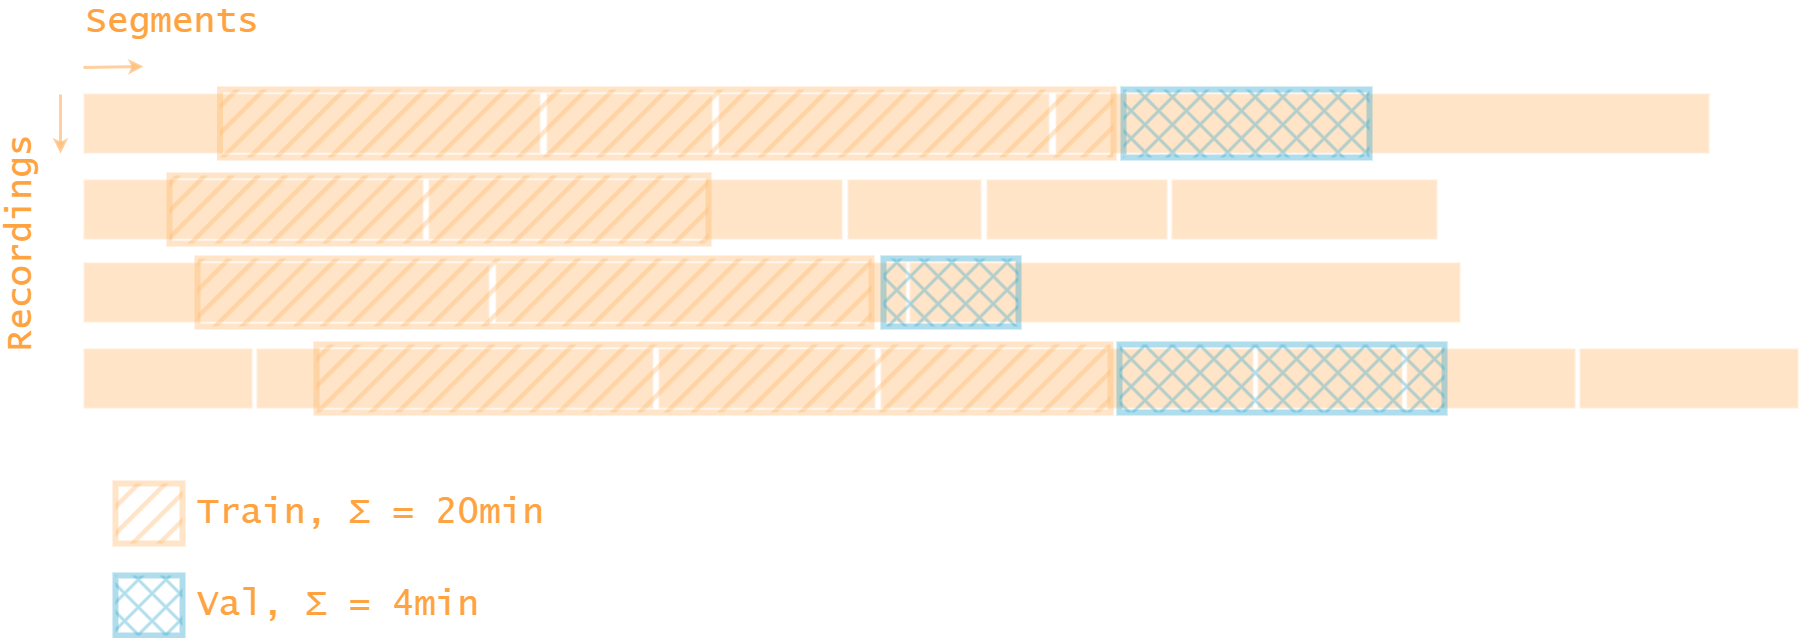
\includegraphics[width=1.0\textwidth]{split.drawio.png}
    \caption{Data Split.}
    \label{fig:split}
\end{figure}

Unlike our required goal, even within the same session the EMG2Pose corpus contains many short recordings of discrete stage classes.
To evaluate \emph{inter-subject} generalization we apply the time-budget logic \emph{per recording}, ensuring every stage class contributes
a training slice and a validation slice:

\begin{itemize}
  \item We aim to carve out generous, non-overlapping intervals -- 
        e.g.\ \texttt{train\_length} = \SI{20}{min} and
        \texttt{val\_length} = \SI{4}{min}.
        Even if a recording is severely segmentated, each interval still contains enough usable footage.

  \item For each recording $r_{i}$ (and thus for each subject), draw  
        a random offset, then cut
        \texttt{train\_length}s $\;\to\;$ \emph{train window}
        followed immediately by
        \texttt{val\_length}s $\;\to\;$ \emph{validation window}.

  \item If a recording is too short for both windows, it is skipped; the global
        budgets are re-balanced across the remaining recordings so the overall
        train/val duration is still met.
\end{itemize}

Because the same seconds-based budgets are enforced for \emph{every} recording,
each subject (stage class) is represented evenly in both splits, satisfying the
inter-subject evaluation goal. Coupled with the "long-window $\to$ fixed-patch
subset $\to$ per-epoch draw strategy, this produces a deterministic,
size-matched pipeline that is fair both \emph{within} EMG2Pose and \emph{between}
EMG2Pose and our single-record dataset.

\subsection{Handling discontinuities and patch sampling.}

\begin{figure}[H]
    \centering
    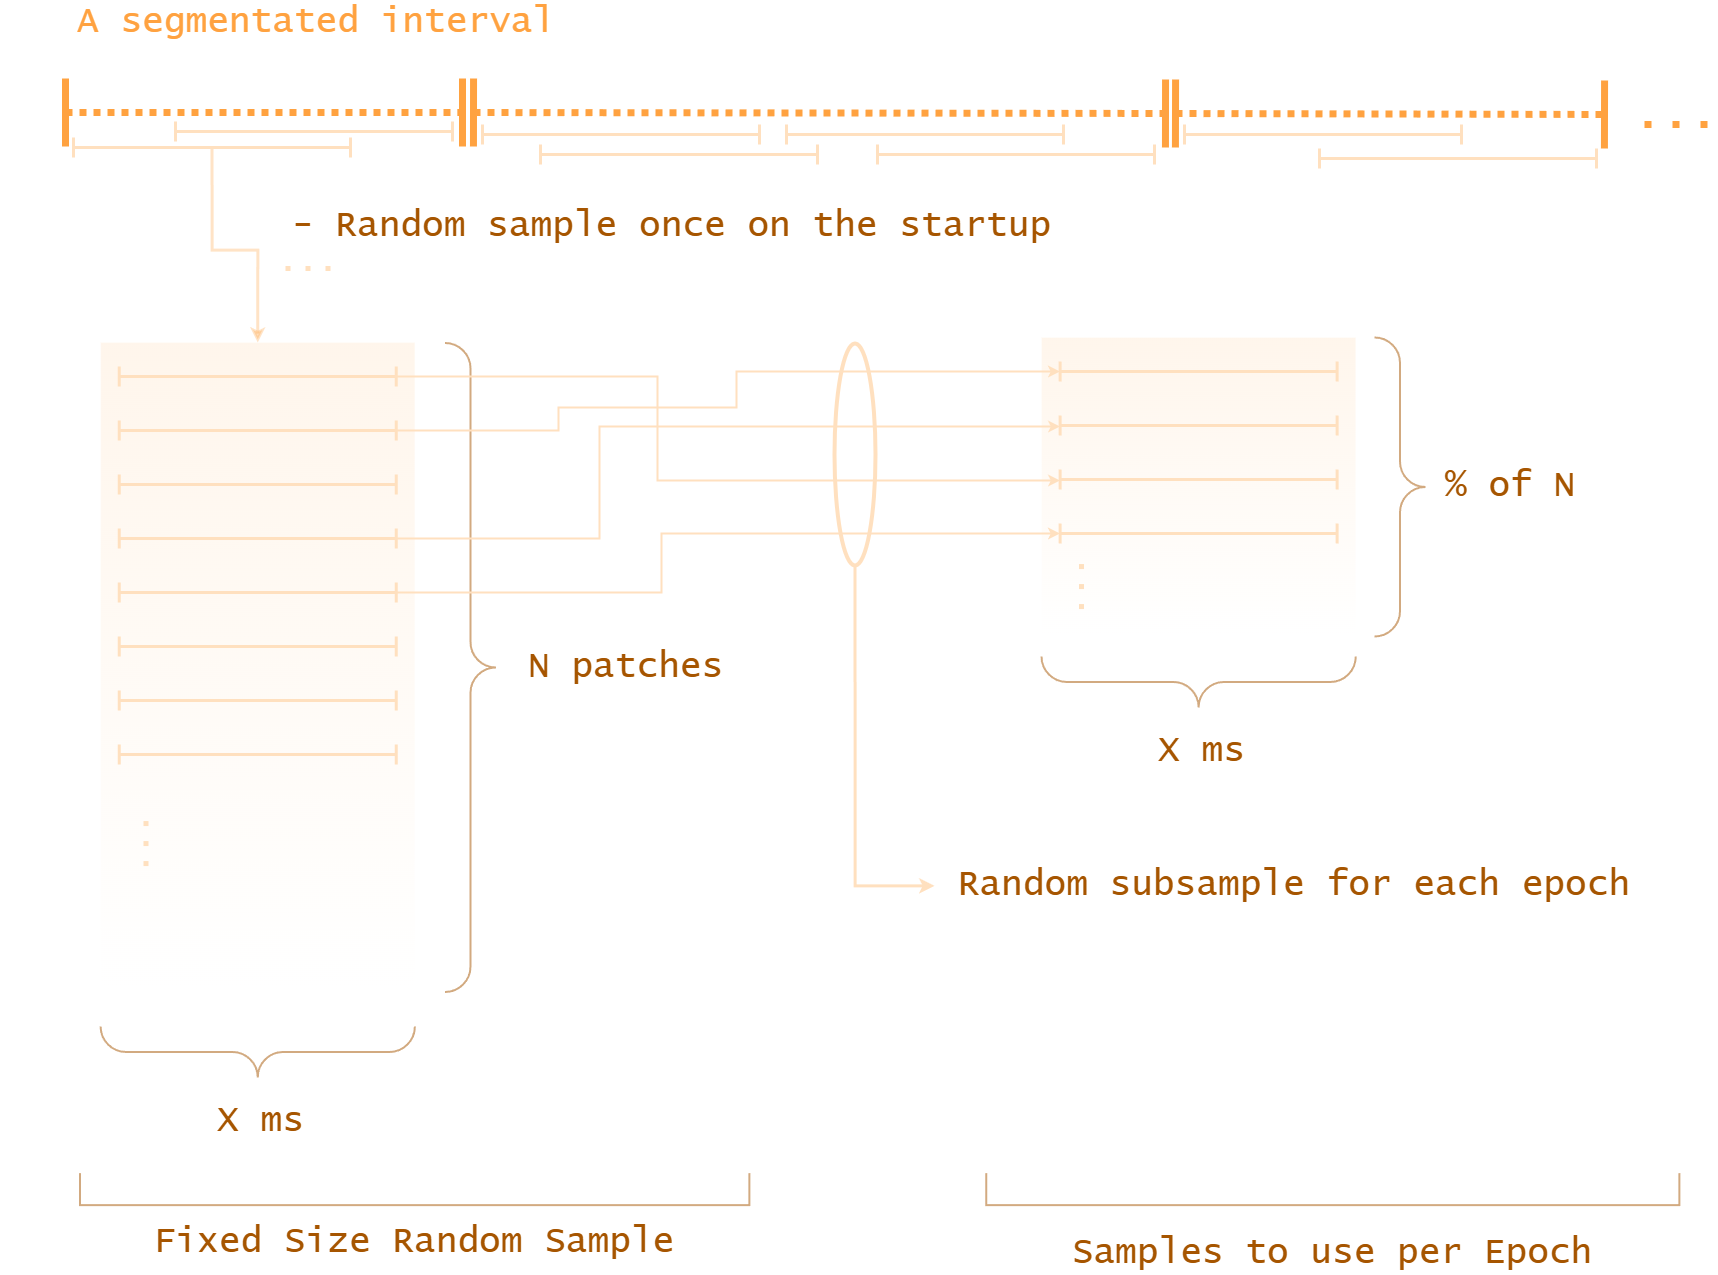
\includegraphics[width=1.0\textwidth]{datasampling.drawio.png}
    \caption{Data Sampling.}
    \label{fig:datasampling}
\end{figure}

Real-world recordings -- especially those in EMG2Pose -- contain brief drop-outs:
marker occlusions, IK failures, or EMG glitches that break a take into smaller
\emph{segments}. If we naïvely extracted every possible 2-second patch from a
long train/val window, datasets with many discontinuities would yield fewer clips, biasing model comparison.

To keep evaluations fair across both our \emph{single, continuous} recording and the \emph{multi-segment} EMG2Pose corpus, we adopt random sampling to keep the number of patches fixed no matter of segmentation, further the subsampling can be applied to reduce the amount of computation per each epoch so a two-tier sampling strategy appears:

\begin{enumerate}[label=\arabic*.]
  \item \textbf{Fixed patch subset.}
        From each long interval we enumerate every admissible 2-second patch
        (sliding by one frame).
        We then \emph{randomly select a fixed number} of patches
        (\texttt{train\_patches}, \texttt{val\_patches}) -- the same count for
        every dataset run.
        This normalises the effective sample size: EMG2Pose and our dataset
        each contribute the identical number of train/val clips, regardless of
        how fragmented the underlying footage is.

  \item \textbf{Per-epoch sub-sampling.}
        During validation or training, only a percentage
        (\texttt{train\_sample\_ratio}, \texttt{val\_sample\_ratio}) of that
        fixed patch pool is drawn each epoch.
        The subset is reshuffled every epoch (with a deterministic RNG seed per
        run) to improve stochastic coverage without changing the overall clip
        inventory.

\end{enumerate}

This three-step approach -- long windows, fixed patch subset, per-epoch draw -- means
that:

\begin{itemize}
  \item A dataset with dense discontinuities (EMG2Pose) and one that is
        nearly continuous (ours) still contribute \emph{exactly the same}
        number of training and validation clips, eliminating bias from
        uneven patch counts.
  \item Stochastic diversity is preserved across epochs, helping optimization,
        yet the total pool remains constant, keeping cross-model metrics
        strictly comparable.
\end{itemize}

\section{Learning Architecture}

Model sources are available at \href{https://github.com/Senopiece/hand_emg_regression/tree/v1.0}{this repository}\footnote{\url{https://github.com/Senopiece/hand_emg_regression/tree/v1.0}}.

\subsection{Interface and Autoregressive Tracking}

\begin{figure}[H]
    \centering
    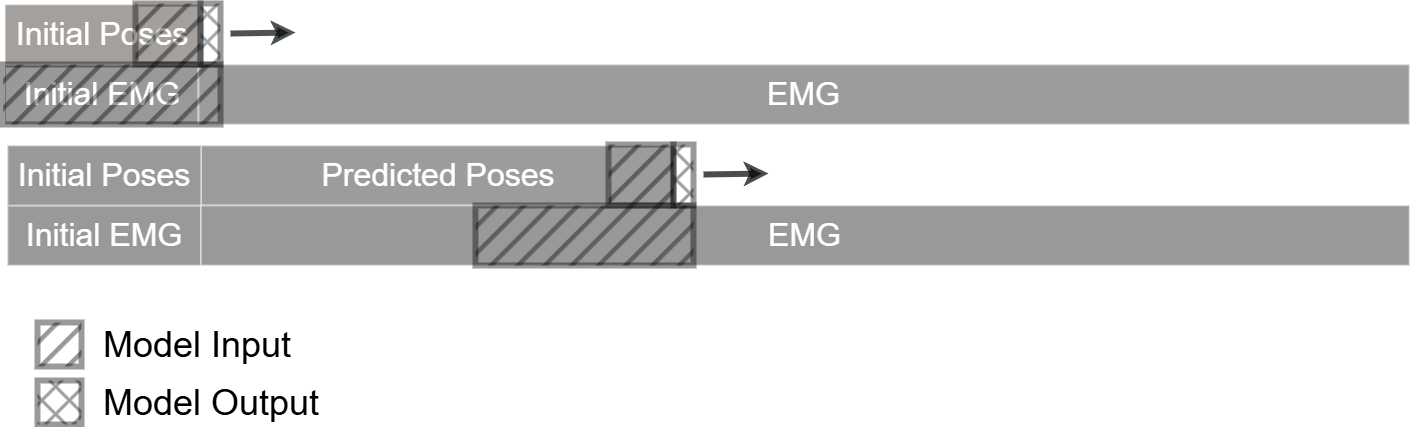
\includegraphics[width=1.0\textwidth]{tracking.drawio.png}
    \caption{Tracking.}
    \label{fig:tracking}
\end{figure}

The network operates on a rolling window of sensory history.
At every step it receives

\begin{itemize}
  \item a \emph{static snapshot} of the most recent EMG slice
        (tens of milliseconds long, covering multiple muscle bursts), and
  \item a \emph{pose context} consisting of the last several hand poses.
        At sequence start these poses come from ground-truth; after the first
        prediction they are replaced by the model`s own outputs.
\end{itemize}

As soon as a new pose is produced, the context window slides forward by one
frame: the oldest pose is discarded, the freshly predicted pose is appended,
and the next EMG slice is read.
Because this loop has no internal state other than the sliding window itself,
tracking can continue indefinitely on a live EMG stream.

\subsection{Next Pose Prediction}

TODO: image

\begin{enumerate}[label=\arabic*.]
  \item \textbf{EMG featuriser}.
        Raw multi-channel EMG is transformed into a dense activation vector.
        Two interchangeable stems are explored.
        The first is a compact 1-D CNN that captures local temporal patterns;
        the second is an adaptive \emph{Spatiotemporal-Sampling} (STS) stem that
        learns both where and when to attend within the EMG slice.
  \item \textbf{Context fusion}.
        The EMG feature vector is concatenated with a flattened summary of the
        pose window-positions, first differences (velocity) and second
        differences (acceleration). This stacked vector forms a rich snapshot
        of "what the hand is doing now" and "how fast it is changing".
  \item \textbf{Stateless predictor}.
        A lightweight multilayer perceptron maps the fused snapshot to the
        next-frame pose. Skip connections inject the velocity-acceleration
        sub-vector at multiple depths inside the MLP, ensuring high-frequency
        motion cues are preserved even after several nonlinear transformations.
        These shortcuts stabilise training and help the network respond quickly
        to abrupt muscle activations.
  \item \textbf{Jitter filter}.
        The raw prediction is combined with the existing pose context by a
        learnable causal filter-effectively a content-aware moving average
        whose weights are trained alongside the rest of the network. The
        filter damps frame-to-frame noise without introducing noticeable lag.
\end{enumerate}

\subsection{Sequence-level Training Objective}

Training is performed on short sequences (e.g.\ a two-second EMG clip).
Within each sequence the network steps forward autoregressively, updating its
own context exactly as it would at run time. Only after the entire rollout is
finished is the composite loss evaluated:

\begin{align*}
\mathcal{L} =\;&
\underbrace{k_0\mathrm{MSE}_{\text{lm}}(\hat L, L)}_{\text{landmark position}} \\
&+ \underbrace{k_1\mathrm{MSE}_{\text{lm}}(\Delta \hat L, \Delta L)}_{\text{velocity}} \\
&+ \underbrace{k_2\mathrm{MSE}_{\text{lm}}(\Delta^{2} \hat L, \Delta^{2} L)}_{\text{acceleration}} \\
&+ k_3\text{L}_{1} + k_4\text{L}_{2}
\end{align*}

Here \(L(\cdot)\) denotes 3-D landmarks recovered via a forward-kinematics layer
compatible with the chosen pose format. $\text{L}_{1} / \text{L}_{2}$ are standard Lasso and Ridge terms. The positional term drives spatial
accuracy, while the velocity and acceleration terms penalize jitter and
encourage dynamical consistency. Parameter regularization keeps the model
compact and reduces over-fitting.
Optimization uses plain gradient descent; because the network is stateless
apart from its sliding window, no back-propagation through time is required.

\medskip\noindent
In summary, the model marries a learnable EMG encoder, a skip-connected MLP,
and a causal filter into a fully autoregressive hand-pose tracker that can
consume continuous EMG data and produce anatomically plausible joint angles in
real time.

\subsection{Comprehensive hyper-parameter sweep}

To put both featuriser families-CNN and STS-on an equal footing, we perform a
single, unified sweep on the Weights\&Biases (W\&B) platform.
A Bayesian optimizer proposes configurations; each proposal trains under a
\emph{Hyperband} early-stopping regime (a run must survive 70 iterations to
avoid pruning and is forcibly stopped at 300).
Mean 3-D landmark error on a fixed validation split is the metric to minimize.

\paragraph{Validation slice (fixed for fairness).}
Regardless of dataset origin, every trial is evaluated on exactly

\begin{itemize}
  \item \textbf{36 seconds of validation footage} drawn from each recording;
  \item a \textbf{2-second prediction horizon} inside that slice;
  \item \textbf{256 validation patches}, of which half are sampled each epoch
        to keep run-time reasonable while leaving the pool unchanged.
\end{itemize}

Locking these numbers removes bias due to clip density or recording length
differences.

\paragraph{Data budget and temporal resolution (swept).}
Conversely, the optimizer may vary how much \emph{training} footage it sees and
at what cadence:

\begin{itemize}
  \item \textbf{Training slice duration}: \SIlist{5;8;12;20;25;30}{min};
  \item \textbf{Prediction horizon during training}: \SIlist{1;2;3;4}{s};
  \item \textbf{Number of training patches}: 7 000 to 200 000;
  \item \textbf{Epoch-sampling ratio}: \SIlist{1;5;10;20}{\%};
  \item \textbf{EMG samples per video frame}: \{16, 32, 64\}
        (\(\approx\)\SIlist{0.25;0.5;1}{ms} resolution per sample).
\end{itemize}

\paragraph{Loss weighting and regularisation.}
The sweep also searches:

\begin{itemize}
  \item \textbf{Position / velocity / acceleration weights}
        (\(\kappa_{\text{pos}},\kappa_{\text{vel}},\kappa_{\text{acc}}\))
        in \{0.1, 1, 10\};
  \item \textbf{L\(_\mathbf{1}\) and L\(_\mathbf{2}\)} regularizers in
        \(\{0,10^{-4},10^{-3},10^{-2},10^{-1},1\}\);
  \item \textbf{Learning-rate} for Adam in \(\{10^{-2},10^{-3},10^{-4}\}\).
\end{itemize}

\paragraph{Pose context and shared MLP widths.}
The size of the sliding pose window and the capacity of the fully connected
stack are treated symmetrically for both stems:

\begin{itemize}
  \item \textbf{Poses in context}: \{3, 4, 8, 12, 20\};
        velocities and accelerations are derived on-the-fly, so a longer
        window provides richer dynamics at the cost of more parameters.
  \item \textbf{Layer widths} for the synapse MLP, muscle MLP, and predictor
        hidden layer: \{32, 64, 128, 512, 1024\}.
        Skip connections re-inject \((\text{pose},\dot{\text{pose}},
        \ddot{\text{pose}})\) vectors at each depth regardless of the width
        chosen.
\end{itemize}

\paragraph{STS-specific search axes.}
The adaptive Spatiotemporal-Sampling encoder adds:

\begin{itemize}
  \item \textbf{Number of temporal slices} and \textbf{patterns per slice}:
        \{4, 8, 16, 32, 128, 256\};
  \item \textbf{Slice width / stride}: \SIrange{8}{800}{ms};
  \item \textbf{Max / Std window width / stride}:
        \SIrange{1}{512}{ms}.
\end{itemize}

\paragraph{CNN-specific search axes.}
When the stem is a conventional 1-D CNN, three kernel lengths are swept:

\begin{itemize}
  \item First convolution, second convolution, and output convolution are each
        drawn from 32 - 1024 samples range,
        spanning fine spike detection to half-second envelopes.
\end{itemize}

\paragraph{Dataset mixing and randomisation.}
At launch, random dataset resolver assembles a fresh session list that blends our own
continuous capture with randomly chosen EMG2Pose sessions.
Consequently, each hyper-parameter set is vetted on \emph{the full diversity of
subjects, hardware, and motion styles}.
A fixed random seed ensures reproducibility-identical W\&B IDs rerun the same
training itinerary-while still exposing the optimiser to representative
variance.

In total, millions of theoretical combinations collapse to a practical number
of trials thanks to Hyperband`s pruning: only promising regions of the search
space are explored deeply, and unpromising ones are terminated early, yielding
a compute-efficient yet thorough search.

\paragraph{Post-sweep model selection and comparative analysis.}
Once the sweep has matured and convergence is observed across multiple promising
trials, we terminate the hyper-parameter exploration and extract the top
configurations for both featuriser families -- STS and CNN.

These best-performing configurations are then \emph{frozen} to ensure that
subsequent comparisons are not biased by additional tuning. With these fixed
architectures and hyperparameters, we proceed to a broader evaluation on
multiple sessions to study the behavior of each model type in various
conditions.

Specifically, we measure:

\begin{itemize}
  \item generalisation across different subject anatomies;
  \item stability on long-form continuous recordings;
  \item sensitivity to underactuated or noisy EMG input segments.
\end{itemize}

This phase allows us to qualitatively and quantitatively assess which featuriser
is better suited to which conditions -- for instance, whether CNNs outperform on
structured gestures, while STS provides robustness to fine-grained spontaneous
motion.

\paragraph{Ablation: EMG-free autoregression.}
To test the hypothesis that hand pose sequences may be partially predictable
even without EMG input -- e.g., due to biomechanical continuity -- we run a
controlled ablation:

\begin{itemize}
  \item The model is provided with an initial sequence of hand poses (and their
        derivatives), but no EMG context at all.
  \item It then autoregressively predicts the next poses solely from its own
        predictions.
  \item Losses are measured against ground-truth pose trajectories.
\end{itemize}

We repeat this test for both our dataset and EMG2Pose recordings.
Performance degradation in this setting quantifies how much of the hand motion
is learnable from kinematic continuity alone -- and by contrast, how much is
uniquely contributed by EMG signals.

This final comparative round, built atop the validated hyperparameter regimes,
provides a holistic view of model expressiveness, sensitivity, and the value of
multimodal input.
